\documentclass[8pt,a4paper]{article}
\usepackage[margin=0.8in]{geometry}
\usepackage[utf8]{inputenc}
\usepackage{amsmath}
\usepackage{amsfonts}
\usepackage{amssymb}
\usepackage[hidelinks]{hyperref}
\usepackage{float}

%s comments
\usepackage{verbatim}

%inline graphs
\usepackage{wrapfig}
% multiple figures on line
\usepackage{subfig}

\usepackage{graphicx}
\graphicspath{ {img/} }

% Caption font size
% https://tex.stackexchange.com/questions/86120/font-size-of-figure-caption-header
\usepackage[font=scriptsize,labelfont=bf]{caption}

\usepackage{fancyhdr}
\pagestyle{fancy}
\lhead{\rightmark}
\chead{}
\rhead{SOFT354 - Parallel Computing and Distributed Systems}
\lfoot{\thepage}
\cfoot{}
\rfoot{Ben Lancaster 10424877}

\renewcommand{\subsectionmark}[1]{\markright{\thesubsection\ #1}}

\begin{document}

\begin{titlepage}
\begin{center}

\vspace*{3cm}
\Large
\textbf{SOFT354 - Parallel Computing and Distributed Systems}

\vspace{0.4cm}
\large
A comparison of the Discrete Fourier Transform algorithm implemented in CUDA and MPI.

\vspace{4cm}
\textbf{Ben Lancaster}\\
\today

\vspace{4cm}
\textbf{Abstract}\\
\small
My placement as a Firmware Engineer at Spirent, a world leader in GNSS simulators. Coming from a Computer Science I was up to speed on the programming aspect of firmware, however was lacking in experience of electronic lab equipment. Constant exposure to this new area of technology and equipment has greatly improved my knowledge in GNSS and embedded programming and has influenced my future career choices. I was chiefly responsible for writing a new programmable timer, implementing fan-control strategies and power calibration schemes, writing a driver to read in peripheral devices, provisioning a Linux hypervisor, and designing and implement a Linux USB driver.

\end{center}

\end{titlepage}

\renewcommand*\contentsname{Table of Contents}
\tableofcontents
\newpage

\section{Introduction}
This report discusses the implementation and performance of the Discrete Fourier Transform (DFT) algorithm in CUDA and MPI.

DFT is largely used in digital signal and image processing applications. 

In this report, I will be implementing the DFT to convert signals in the time domain to the frequency domain.


\begin{figure}[H]%
    \centering
    \subfloat[Time domain]{{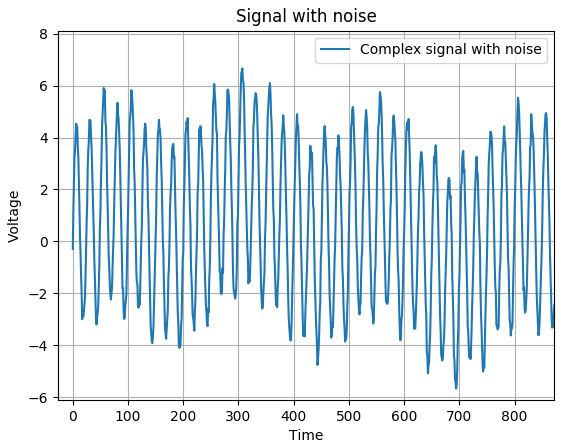
\includegraphics[width=7cm]{intro_signal} }}%
    \qquad
    \subfloat[Frequency domain]{{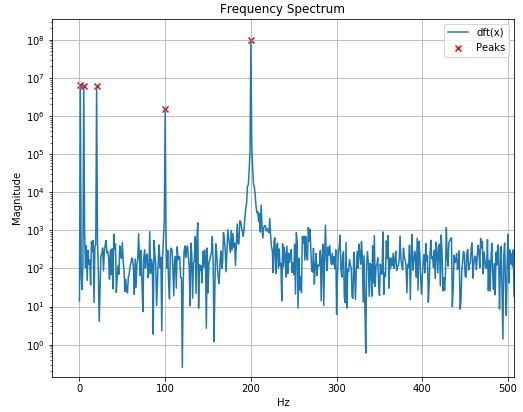
\includegraphics[width=7cm]{intro_dft} }}%
    \vspace{5pt}
    \caption{\textbf{Left:} A compound signal made up of 1, 5, 20, 100, and 200 Hz sine waves in the time domain. \textbf{Right:} Frequency domain representation showing high amplitude peaks for the 1, 5, 20, 100, and 200 Hz waveforms.}%
    \label{fig:gridwatch}%
\end{figure}

\section{Implementation}
\subsection{CUDA}

\subsubsection{Dynamic Shared Memory}
As each operation on each sample requires values from all other samples, global memory accesses will be largest performance bottleneck. To reduce the amount of global memory accesses, I had the first thread of each block copy the complete global memory copy of the samples to a local shared memory buffer, which the DFT kernel would access instead of the global memory. 

\begin{wrapfigure}{r}{0.4\textwidth}
\begin{center}
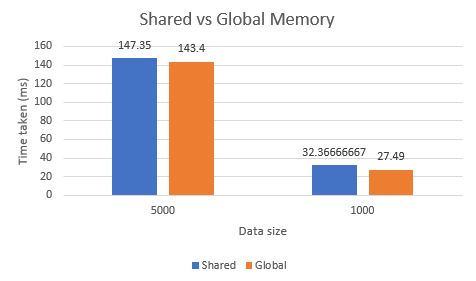
\includegraphics[scale=0.6]{shared_vs_global_graph}
\end{center}
\caption{Average kernel execution time using shared vs. global memory.}
\label{fig:shared_vs_global_graph}
\end{wrapfigure}
On Compute Capability 2.0 devices, the maximum shared memory size per block is 48KB, meaning that if the kernel was launched with 1 block, it could access all 48KB of memory. If two blocks were used, each block would have 24KB of memory. 

To be able to fit the entire sample set in shared memory, I had to keep the maximum shared memory per block at it's highest by using as few blocks as possible. I used the maximum of 1024 threads per block to reduce the number of required blocks.  

Using any number of 8-byte samples below 2048, which would use up to 2 blocks of 1024 threads and 24KB of shared memory, allows all samples for each block to fit into their shared memory. 

If using more than 2048 8-byte samples, resulting in using 3 or more blocks, results in the shared memory per block overflowing. The kernel handles this by pausing blocks that do not have enough shared memory ready, and running blocks that do have all their shared memory ready.

Even though we are accessing faster memory, it's size limitations causes resource availability delays when using larger data sets, which results in higher latency and lower performance. 


\subsection{MPI}
With DFT, each sample must have operate on all other samples. In my implementation, I must first copy the complete sample array to each node. 

\begin{figure}[H]
\begin{center}
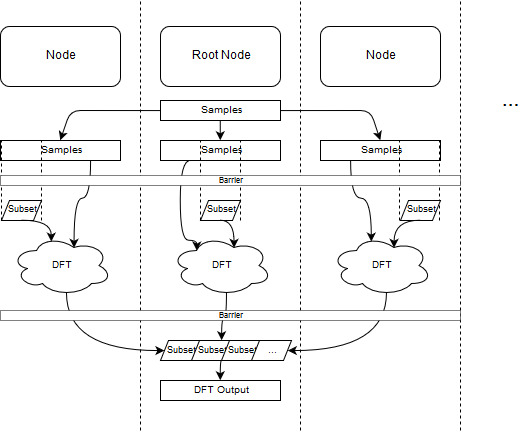
\includegraphics[scale=0.7]{mpi_impl1}
\end{center}
\caption{Control flow diagram for the MPI DFT algorithm.}
\label{fig:train10x}
\end{figure}

\section{Evaluation}
\subsection{Measuring Performance}


\end{document}
